% Cria um novo contador para modificar o mecanismo de label
% e o comando \ref{} funcionar de maneira correta.
% https://tex.stackexchange.com/questions/62742/how-to-label-ref-an-un-numbered-section
\newcounter{anexo}

\newcommand{\titulo}{ANEXO A - Lorem Ipsum}
\chapter*{\titulo}

	% Esses comandos corrigem o comando \ref{}.
	\renewcommand{\theintro}{A}
	\refstepcounter{anexo}
	\label{anexoA}
	\addcontentsline{toc}{chapter}{\titulo} % Adiciona o apêndice na table of contents.

  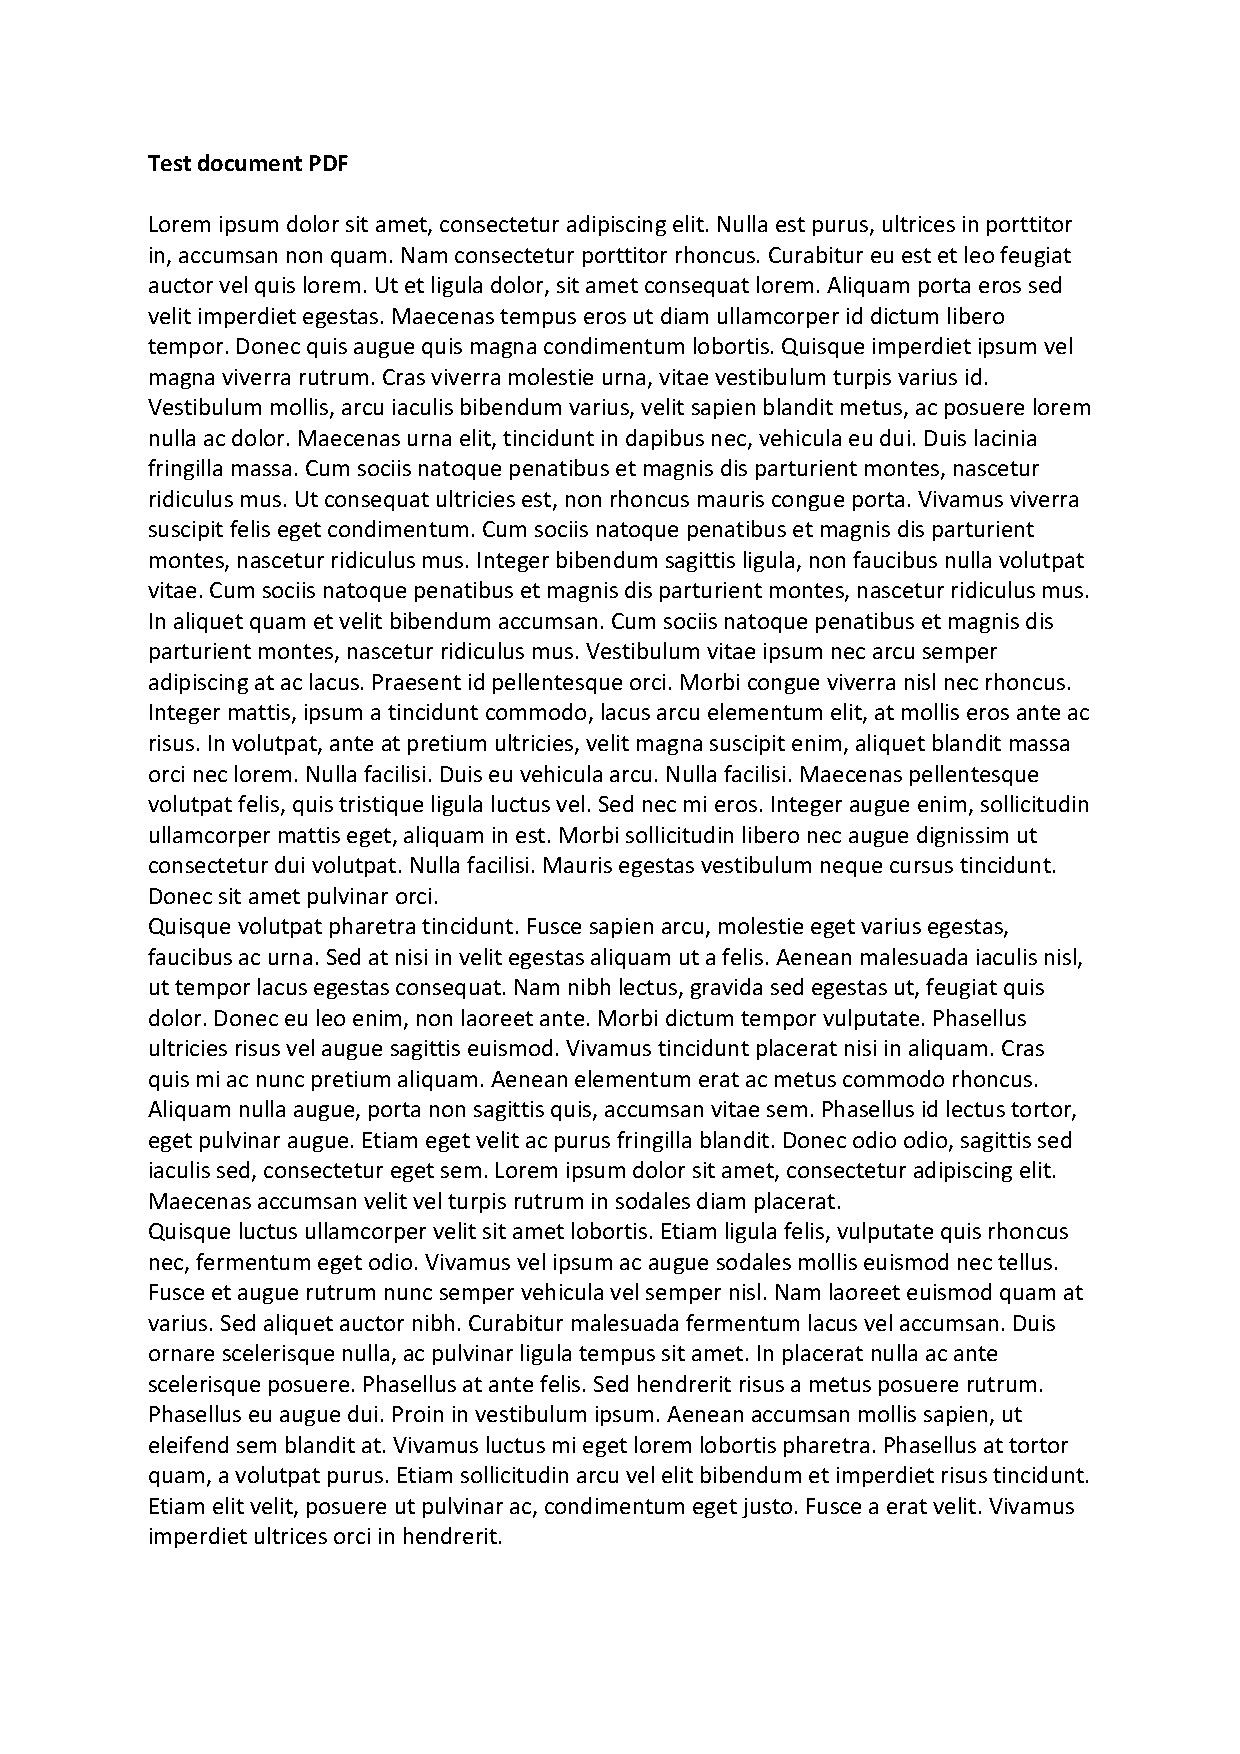
\includepdf[angle=0, scale=1, pages=-]{anexos/lorem-ipsum.pdf}
